\chapter{Introduction}
\labch{introduction}

Recent advances and evolution in software development have made software more and more complex.
The reliability of software systems is based on their correctness.
Any failure or vulnerability in software poses a significant risk, potentially threatening human safety or causing financial losses.
As software systems become more complex, also the likelihood of bugs increases.
The effort and cost to fix these bugs escalate with late detection, \reftab{effort-to-fix} illustrates the relative costs of fixing bugs at different development stages.
Nowadays, software rules safety-critical systems such as nuclear power plants, car engines, airplane control systems, and medical devices.
For system where safety is critical, addressing bugs before deployment is mandatory.

\begin{margintable}[*1]
  \caption{Cost to fix bugs at different development stages.}
  \labtab{effort-to-fix}
  \centering
  \resizebox{\textwidth}{!}{
  \begin{tabular}{r r}
    \toprule
    \textsc{Bug Found at Stage} & \textsc{Cost to Fix} \\
    \midrule
    Requirements & 1x (definition) \\
    Architecture & 3x \\
    Design & 5-10x \\
    System Test & 10x \\
    Production & 10-100x \\
    \bottomrule
  \end{tabular}
  }
\end{margintable}

Nowadays, machine learning software has an ever-increasing societal impact by assisting or even automating decision-making in fields such as social welfare, criminal justice, and even health care.
At the same time, a number of recent cases have shown that such software may reproduce, or even reinforce, bias directly or indirectly present in the training data \sidecite[*4]{BuolamwiniGebru2018,KayMatuszek2015,COMPAS,ObermeyerPowers2019}.
In April 2021, the European Commission proposed a first legal framework on machine learning software -- the Artificial Intelligence Act~\sidecite[*12]{ArtIntAct}
--- which imposes strict requirements to minimize the risk of discriminatory outcomes.

Moreover, recent advancements in artificial intelligence have led to the rise of large language models (LLMs) capable of generating software from natural language specifications. Agents like OpenAI's ChatGPT and Google's Gemini are gaining widespread use. Specifically designed for coding, GitHub Copilot assists programmers within IDEs and has over a million subscribers. Despite their benefits, AI-generated code can introduce as many bugs as human-written code, making it crucial to use techniques that detect software errors or certify intended behaviors.

\section{Software Quality}

Software quality is a measure of how well software meets its requirements.
The most common method to ensure software quality is \emph{testing}.
The correct behavior of software is tested empirically for finite number of inputs against a set of assertions that specify the functional requirements of the code.
However, testing has inherent limitations.
Testing can only verify a program against the functional requirements, which may be poorly defined and ambiguous, leading to inadequate testing.
Exhaustive testing of systems is impractical, and constraints on time and budget can further impact the process.
But mostly, testing is not sufficient to guarantee the absence of bugs in software\sidenote{``program testing can be quite effective for showing the presence of bugs, but is hopelessly inadequate for showing their absence.'' -- Edsger W. Dijkstra} \sidecite{Dijkstra1976}.
While in some cases it is acceptable to deploy software with bugs (and rely on patches to fix them, \reftab{effort-to-fix}), in the case of safety-critical systems, it is necessary to ensure that the software is free of bugs before deployment to avoid catastrophic consequences.

In contrast, \emph{formal methods} provide rigorous mathematical guarantees about the correctness of software.
Thanks to their mathematical foundation, an approach based on formal methods guarantees 100\% accuracy in the verification of software properties.
The idea of formally verifying software is not new, and it has been around since the late 1960s with program proofs and invariants from \sidetextcite{Floyd1967} and \sidetextcite{Hoare1969}.
Even before, formal methods may be traced back to the work of \sidetextcite{Church1936} and \sidetextcite{Turing1936} on the foundations of computation.
According to software engineering practices, formal methods can be introduced early in the development lifecycle, enabling the verification of software properties at the design stage.
%
\begin{center}\em
  Why should formal methods replace other well-known, widely accepted, and user-friendly techniques such as testing?
\end{center}
To answer this question, we provide examples where testing failed.


Ariane 5 rocket failure\sidenote{\url{https://esamultimedia.esa.int/docs/esa-x-1819eng.pdf}} in 1996 caused by an integer overflow bug resulting in a loss of \$370 million.
Airfrance Flight 447 crashed in June 2009, killing hundreds of passengers, due to a probe sensor that were not able to accurately measure the airplane speed, which in turns disengaged the autopilot. The probe fault was not detected during testing as the test engineers assumed that such an event was impossible to happen.
Similarly, the Therac-25 radiation therapy\sidecite{Leveson1993} machine where at least six patients received massive overdoses of radiation due to race conditions.
The Toyota unintended acceleration\sidenote{\url{https://www.embeddedrelated.com/showarticle/1574.php}} case where a stack overflow resulted in the death of 89 people and a lawsuit of \$1.2 billion.
The roundoff error in the Patriot missile system\sidenote{\url{https://www.ima.umn.edu/~arnold/disasters/patriot.html}} that caused the death of 28 people during the Gulf War.
All these cases could have been avoided with formal methods.

Unlike testing, formal methods enable exhaustive investigation and detection of bugs that testing may miss. The actual system requirements are translated into formal specifications, which are mathematically verified to ensure the system's behavior aligns with real-world scenarios.
However, Rice's undecidability theorem \sidecite{Rice1993} states that all non-trivial properties\sidenote{
  A property is non-trivial if it is not true for all programs or false for all programs.
} are undecidable, which means that there is no terminating algorithm that can decide whether a program satisfies a non-trivial property.
Therefore, as a consequence of Rice's theorem, formal methods either sacrifice \emph{completeness}, \emph{soundness}, or \emph{automation}.
Current formal methods can be classified into three categories\sidecite{Cousot2010}: \emph{theorem provers}, \emph{model checking}, and \emph{static analysis}.



\begin{marginfigure}
  \centering
  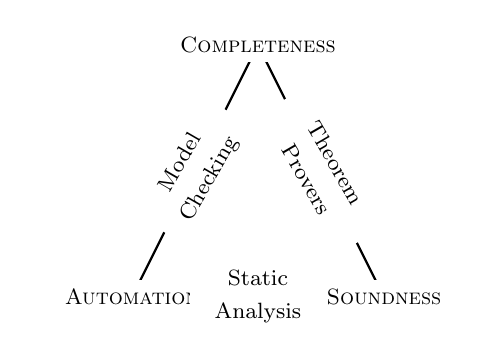
\begin{tikzpicture}[scale=0.8]
    % Draw the triangle
    \draw[thick] (0,0) -- (4,0) -- (2,4) -- cycle;

    % Place the vertices with blue squared borders
    \node[draw, fill=white, text width=2.4cm, align=center, draw=white] at (0,0) {\footnotesize \textsc{Automation}};
    \node[draw, fill=white, text width=2cm, align=center, draw=white] at (4,0) {\footnotesize \textsc{Soundness}};
    \node[draw, fill=white, text width=2.6cm, align=center, draw=white] at (2,4) {\footnotesize \textsc{Completeness}};

    % Place the edges' labels inside the edges
    \node[fill=white, text width=1.5cm, align=center] at (2,0) {\footnotesize Static Analysis};
    \node[fill=white, text width=1.5cm, align=center, rotate=60] at (1,2) {\footnotesize Model Checking};
    \node[fill=white, text width=1.8cm, align=center, rotate=-60] at (3,2) {\footnotesize Theorem Provers};
\end{tikzpicture}
  \caption{Trade-offs in formal methods.}
  \labfig{formal-methods-trade-offs}
\end{marginfigure}

Theorem provers produce proofs of correctness employing interactive tools, also called proof assistants, such as Coq, Isabelle, and HOL Light, or automatic ones like \dots
Ultimately, user interaction is required to guide the proof search.
Even in automatic theorem provers, where automation is key design, to verify any general property, user interaction is required at some point.
Theorem provers are complete and sound, but they are not fully automated.

Formal methods based on model checking explore completely and automatically the state space of a program's model to verify whether undesirable states are reachable.
\sidetextcite{Clarke2004} apply model checking to prove the correctness of ANSI-C programs.
However, model checking-based methods are limited by the state explosion problem: since the number of feasible execution paths grows exponentially with the size of the model, this category of formal methods trade soundness for completeness and automation.

Static analysis is a category of formal methods that analyze without user interaction the program source code to some level of abstraction.
This abstraction is sound but incomplete, meaning that the analysis may report \emph{false alarms}, \ie, warnings that a correct program may be incorrect. However, whenever the static analysis certifies the absence of a bug, the program is indeed bug-free.
The most common static analysis techniques are based on \emph{abstract interpretation}.

Abstract Interpretation \sidecite{Cousot1977} is a general theory for approximating the program semantics, developed by Patrick and Radhia Cousot in the late 1970s.
Their framework is based on the observation that to reason about program properties, not all the computational details are necessary.
Instead, the program's semantics can be approximated by a simpler, more abstract model that facilitate the automatic reasoning.

Over the past decade, abstract interpretation-based static analyses have been successfully applied to the development cycle of real-word software.
The \emph{Astrée} static analyzer \sidecite{Cousot2005} is routinely used to ensure the absence of runtime errors in embedded synchronous C programs for the Airbus A340 and A380.

We provide a formal introduction to abstract interpretation in \refch{abstract-interpretation},
and we recall the main results used in this thesis, which are later illustrated
on a small idealized programming language at the end of the same chapter.


\section{Input Data Usage}

In software systems, programming errors do not always result in crashes or runtime errors.
It may be the case that the faulty program produces a plausible yet erroneous outcome or unsafe behavior.
Such bugs are hard to spot since they provide no clear indication that something went wrong.
A potential source of such errors is the misuse of input data, \ie, when an input variable has an unexpected impact on the program computation compared to the developers' expectations.

A notable example is the Reinhart and Rogoff article ``Growth in a Time of Debt'' \sidecite{Reinhart2010}, which claimed that economic growth is negatively correlated with public debt.
This article was heavily cited to justify austerity measures around the world in the following years.
However, in 2013, \sidetextcite{Herndon2013} discovered that the authors had made a mistake in their Excel spreadsheet, which led to the erroneous conclusion.
Notably, one of the several programming and methodological errors discovered is the incorrect usage of the input value relative to Norway's economic growth in 1964, with an excessive weight in the computation of the average growth rate.

Particularly in the context of data science applications, where software involves long pipeline of layers that filter, merge, and manipulate data, the likelihood of programming errors that cause some input variables to be more, or less, in fluent than what was expected is high.
Hence, it is important to employ techniques that enhance the confidence in the usage of input variables for data-driven applications.

\refch{input-data-usage} introduces the input data usage property, which is a formal property that captures the \emph{qualitative} usage of input data in a program.

\section{Quantitative Properties}

Commonly, in the context of properties of programs, a program either satisfies a property or not.
Such qualitative restriction is not sufficient to capture the complexity of real-world requirements.
Consider for instance one of the most fundamental security issues: protecting the confidentiality of sensitive information.
In secure information flow analysis the question is whether a program could leak information about its secrets.
A classic approach, based on any of the formal methods explored above, would try to enforce \emph{noninterference}, certifying that a program reveals no information about its secrets.
Unfortunately, noninterference is too strict for many practical applications.
In the case of a digital election protocol, individual votes should be anonymous, but of course the final result needs to be revealed. A password checker should not reveal the password, but it should reveal whether the password is correct.
These cases represent deliberate violations of noninterference that are necessary for the program to fulfill its purpose.

To address this limitation, one approach is to consider quantitative properties.
The key idea is to accept that a program may violate a property, and compare such violation against a threshold.
Programs are classified as \emph{safe} or \emph{unsafe} based on the degree of violation, thus inducing a classification among programs based on how much safety they provide.


In the Reinhart and Rogoff case, the value of Norway's economic growth was indeed used in the average computation, but its impact was much higher than it should have been.
The error was not whether the value was used or not, but rather how much it was used.
In this case, a quantitative analysis would have revealed that the impact of Norway's economic growth was too high, and the authors could have corrected the wrong conclusion.

\refch{quantitative-input-data-usage} introduces the formal framework, based on abstract interpretation, to reason about quantitative properties of programs of input data usage.


\section{Outline and Contributions}

In this thesis, we study techniques based on formal reasoning to detect misuse of input data.
We propose semantics-based static analysis techniques to soundly quantify the impact of input variables on the program computation.
\refch{abstract-interpretation} provides the mathematical background used in the rest of the thesis and introduces the formal framework of abstract interpretation.

The rest of this section outlines the organization of the main body of this thesis.
\refch{experimental-evaluation} presents the experimental evaluation, \refch{related-work} discusses related work, and \refch{conclusion} concludes the thesis with a summary and future work.

\subsection{Input Data Usage}

In \refch{input-data-usage}, we focus on the definition of the input data usage property. Specifically, we introduce its definition as proposed by \sidetextcite{Urban2018}.
Then, we extend the property to capture abstractions of output values as done in the generalization of non-interference property \sidecite{Giacobazzi2018}.
We provide the hierarchy of semantics that precisely captures the input data usage property abstracting unnecessary details.
Finally, from \textcite{Urban2018} we report an abstract semantics that captures syntactic dependencies between variables, which is used to soundly approximate the input data usage property.

\subsection{Quantitative Input Data Usage}

In \refch{quantitative-input-data-usage}, we present a novel quantitative input usage framework to discriminate between input variables with different impact on the outcome of a program.
This framework can be used to identify variables that have a disproportionate impact.
Such knowledge could either certify intended behavior or reveal potential flaws, by matching the developers' intuition on the expected impact of their input with the actual result of the quantitative study.
We characterize the impact of an input variable with a notion of dependency between variables and the outcome of a program.
In general, determining how an input variable influences a program outcome depends on several factors, such as the structure of the program, the environment, the expertise of the developer, and the intuition of the researcher.
Consequently, there is no single impact definition that fits all requirements. For this reason, our framework is parametric in the impact definition of choice.

Building on this framework, we introduce a backward static analysis based on abstract interpretation parametric in the definition of impact, which automatically infers a sound over-approximation of the impact of input variables when analyzing programs. We design our static analysis to soundly approximates our property, by returning an upper bound on the impact quantity.
The inputs of our static analysis consist of a set of cumulative ranges representing program outputs, called output buckets.
Then, the analysis backward computes the input states leading to these buckets and applies a computable implementation of the impact on the result of the backward reachability analysis.
This approach allows end-users to choose the impact that best fits their needs, ensuring a more targeted and customizable analysis.

In \refsec{showcase-of-outcomes-and-ranges} we demonstrate the potential applications of the quantitative framework by evaluating an automatic conceptual tool of our static analysis, called \impatto, against six use cases: a simplified program from the Reinhart and Rogoff article, a program extracted from the recent OpenAI keynote, three from termination analysis, and a crafted example resembling an aircraft landing alarm system. This chapter is based on work published at NASA Formal Methods Symposium (NFM) 2024 \sidecite{Mazzucato2024nfm}.


\subsection{Quantitative Verification for Neural Networks}

In \refch{quantitative-fairness}, we extend the quantitative input data usage property to the domain of neural networks.
We propose two impact notions for neural networks. The first one addressing the ragged input space of neural networks, and the second one measuring the amount of fairness of input features.
First, we show how a na\"ive approach measures the impact of input features in neural networks, and then we refine the backward analysis to exploit parallel computations and achieve better performance.

Our approach employs a combination of forward and backward analyses.
The forward pass aims to reduce the combinatorial explosion the backward analysis faces when analyzing neural-network models.
The static analysis revolves around the concept of \emph{independent input partitions}, partitioning the input space into subregions that are easier to analyze for the backward analysis and do not interfere with each other, allowing parallel computations.
Moreover, the forward analysis can be configured in terms of scalability and precision to adapt to the user's needs. By the choice of abstract domain and budget of resources, the analysis trades off precision for execution time.
The resource budget can be auto-tuned to find the best analysis configuration according to a given search heuristic.

\refsec{evaluation-on-neural-networks} presents the evaluation of our approach on neural networks.
This chapter is based on work published at the 28th Static Analysis Symposium (SAS) 2021 \sidecite{Mazzucato2021}.

\subsection{Quantitative Static Timing Analysis}

In \refch{quantitative-static-timing-analysis}, we consider the amount of program iterations during the execution of a program as the program outcome.
Thus, we capture the impact of input variables on the \emph{global} number of iterations of a program.
Such variation is interesting as programming errors related to the misuse of input data affecting the number of iterations may degrade performance or introduce security vulnerabilities without even showing any functional error.
For instance, in the context of security, an unexpected impact of input variables on the program's runtime could reveal sensitive information \sidecite{Wong2005}, leading to potential security threats.
Even in cryptography, where programs are mathematically robust, vulnerabilities to timing attacks persist, depending on the implementation choices and design.
\sidetextcite{Kocher1996} demonstrated that widely used public key cryptographic algorithms, like RSA, are vulnerable to timing attacks, and may leak information about the secret key.
The value of such attacks lies in their simplicity;
attackers do not need to possess detailed knowledge of the program implementation or engage in computationally expensive operations.
Merely the information of which primitives are used in the program is enough.
For example, knowledge that the exponentiation operation, commonly found on cryptographic programs, is performed using the square-and-multiply algorithm can enable an attacker to exploit the program's runtime to infer the secret key \sidecite{Wong2005}.
Indeed, \sidetextcite{Dhem2000} mounted such attack against CASCADE smart cards, observing timing differences during the square operations of the square-and-multiply algorithm.
Furthermore, knowing the timing behavior of a program could certify intended behavior or reveal latent flaws by matching developers' expectations with the actual program behavior.
For performance optimization, identifying input variables that most significantly affect loop iterations can help developers focus on critical code segments \sidecite{Omar2017}.
As a consequence, achieving a comprehensive understanding of the impact of input variables on the program runtime is paramount.
In this study we focus on quantifying the impact of input variables on the number of loop iterations in a program, as an indicator of the program's runtime behavior.


In this chapter, we leverage an underlying global loop bound analysis to derive an over-approximation of the global loop bound and encode the quantification of each input variable's impact as a linear programming problem.
Our approach blends syntactic and semantic information:
to improve accuracy, the global loop bound analysis generates invariants as a set of linear constraints;
to improve scalability, we combine the global loop bound analysis with a syntactic dependency analysis \sidecite{Urban2018}, reducing the number of variables to analyze.

In \refsec{showcase-of-outcomes-and-ranges} we present \timesec: a tool that implements our quantitative timing analysis. Our demonstrate the effectiveness of our tool in a real-world library for cryptographic applications. Notably, we certify the library's immunity to timing side-channel attacks by showing that input variables have no impact on loop iterations. Additionally, we evaluate \timesec{} against programs drawn from \svcomp.
This chapter is based on work published at the 31st Static Analysis Symposium (SAS) 2024 \sidecite{Mazzucato2024sas}.

\subsection{Contributions}

The main contributions of this thesis are as follows:
\begin{itemize}
  \item In \refch{input-data-usage}:
  \begin{itemize}
    \item we extend the original definition of the input data usage property to capture abstractions of output values.
    Such extension blends generalized non-interference with input data usage, providing a definition that works also for non-deterministic programs.
  \end{itemize}
  \item In \refch{quantitative-input-data-usage}:
    \begin{itemize}
      \item we develop a theoretical framework by abstract interpretation to quantify the impact of input variables by considering three instances of impact.
      \item we present our static analysis and a possible abstract implementation of the impact instances.
    \end{itemize}
  \item In \refch{quantitative-fairness}:
    \begin{itemize}
      \item we present two impact notions for neural networks.
      \item we propose an improved backward analysis that exploits parallel computations and achieves better precision by combining together abstract domains.
    \end{itemize}
  \item In \refch{quantitative-static-timing-analysis}:
    \begin{itemize}
      \item we propose a static analysis based on abstract interpretation, employing a linear constraint abstract domain, global loop bound analysis, and linear programming encoding to quantify input variable impact on loop iterations.
    \end{itemize}
\end{itemize}
